\documentclass[10pt]{article}

\usepackage{graphicx}
\usepackage{float}
\usepackage{subcaption}

\usepackage{graphicx}
\usepackage{kotex}
\usepackage{amsmath}
\usepackage{amssymb}
\usepackage{float}

\begin{document}

\begin{center}
고급물리 기말 프로젝트
\end{center}

\begin{flushright}
2023017030 채서병
\end{flushright}

1. Henon Map

\begin{equation}
\begin{cases}
x_{n+1}=1-a x_n^2+y_n\\
y_{n+1}=b x_{n}
\end{cases}
\end{equation}

\vspace{1em}

1.1 Dissipative system 
\begin{equation}
J = \begin{vmatrix}
    -2ax_n & 1 \\ b & 0
\end{vmatrix}
\end{equation}

|det J| = b 일때, -1 < b <1 이라면 넓이가 감소하기 때문에 소산계(dissipative system)이다.

\vspace{1em}

1.2 Fixed points

해논 맵에서 각 고정점을 구하면
\begin{equation}
    \begin{cases}
        x^* = 1-a (x^*)^2 + y^* = 1 - a (x^*)^2 + b x^*\\
        y^* = b x^*
    \end{cases}
\end{equation}

식 (3)을 정리하여 \(x^*\)을 구하면

\begin{equation}
    x^* = \frac{(b-1) \pm \sqrt{(1-b)^2 + 4a}}{2a}
\end{equation}

이므로 \((x^*, y^*)\)을 구하면

\begin{equation}
    (x^*_{\pm}, y^*_{\pm}) =-(\frac{(b-1) \pm \sqrt{(1-b)^2 + 4a}}{2a}, b\frac{(b-1) \pm \sqrt{(1-b)^2 + 4a}}{2a})
\end{equation}

이때, 실수 고정점이 존재하기 위해서는 판별식이 0 이상이어야 함으로
\begin{equation}
    (1-b)^2 + 4a \ge 0
\end{equation}

\begin{equation}
    \therefore a \ge \frac{-(1-b)^2}{4}
\end{equation}

이다. 

\vspace{1em}

이제 선형성을 통하여 분석을 하자면 식 (2)의 야고비안에서 고정점을 대입하여 행렬식을 구하면 
\begin{equation}
J = \begin{vmatrix}
    -2ax^* - \lambda & 1 \\ b & -\lambda
\end{vmatrix}
\end{equation}

이를 통하여 구한 특성 방정식은 
\begin{equation}
    \lambda^2 + 2ax^*\lambda -b = 0
\end{equation}
이며, 고정값은
\begin{equation}
    \lambda_{\pm} = -ax^* \pm \sqrt{a^2(x^*)^2 + b}
\end{equation}
이다.

\vspace{1em}

여기서 나온 두 고유값에 대하여 \(|\lambda_1|<1,\  |\lambda_2|<1\)이라는 조건을 만족해야 함으로 b의 조건 또한 \(-1<b<1\)이라는 조건과 
\(|2ax^*| < 1-b\)의 조건을 만족 해야한다.

\vspace{1em}

\(D = \sqrt{(1-b)^2 + 4a}\)라 할때 식 (4)를 이용하여 \(2a x^*_{\pm} = b-1 \pm D\)를 구할 수 있다.
이때 b가 \(-1< b < 1\)에서 \(x^*_{-}\)는 항상 불안정 하다. 반면 \(x^*_+\)는 \(\frac{-(1-b)^2}{4} < a < \frac{3(1-b)^2}{4}\)
일때 안정이다. 

\vspace{1em}

1.3 Numerical simulations
\begin{figure}[H]
\centering
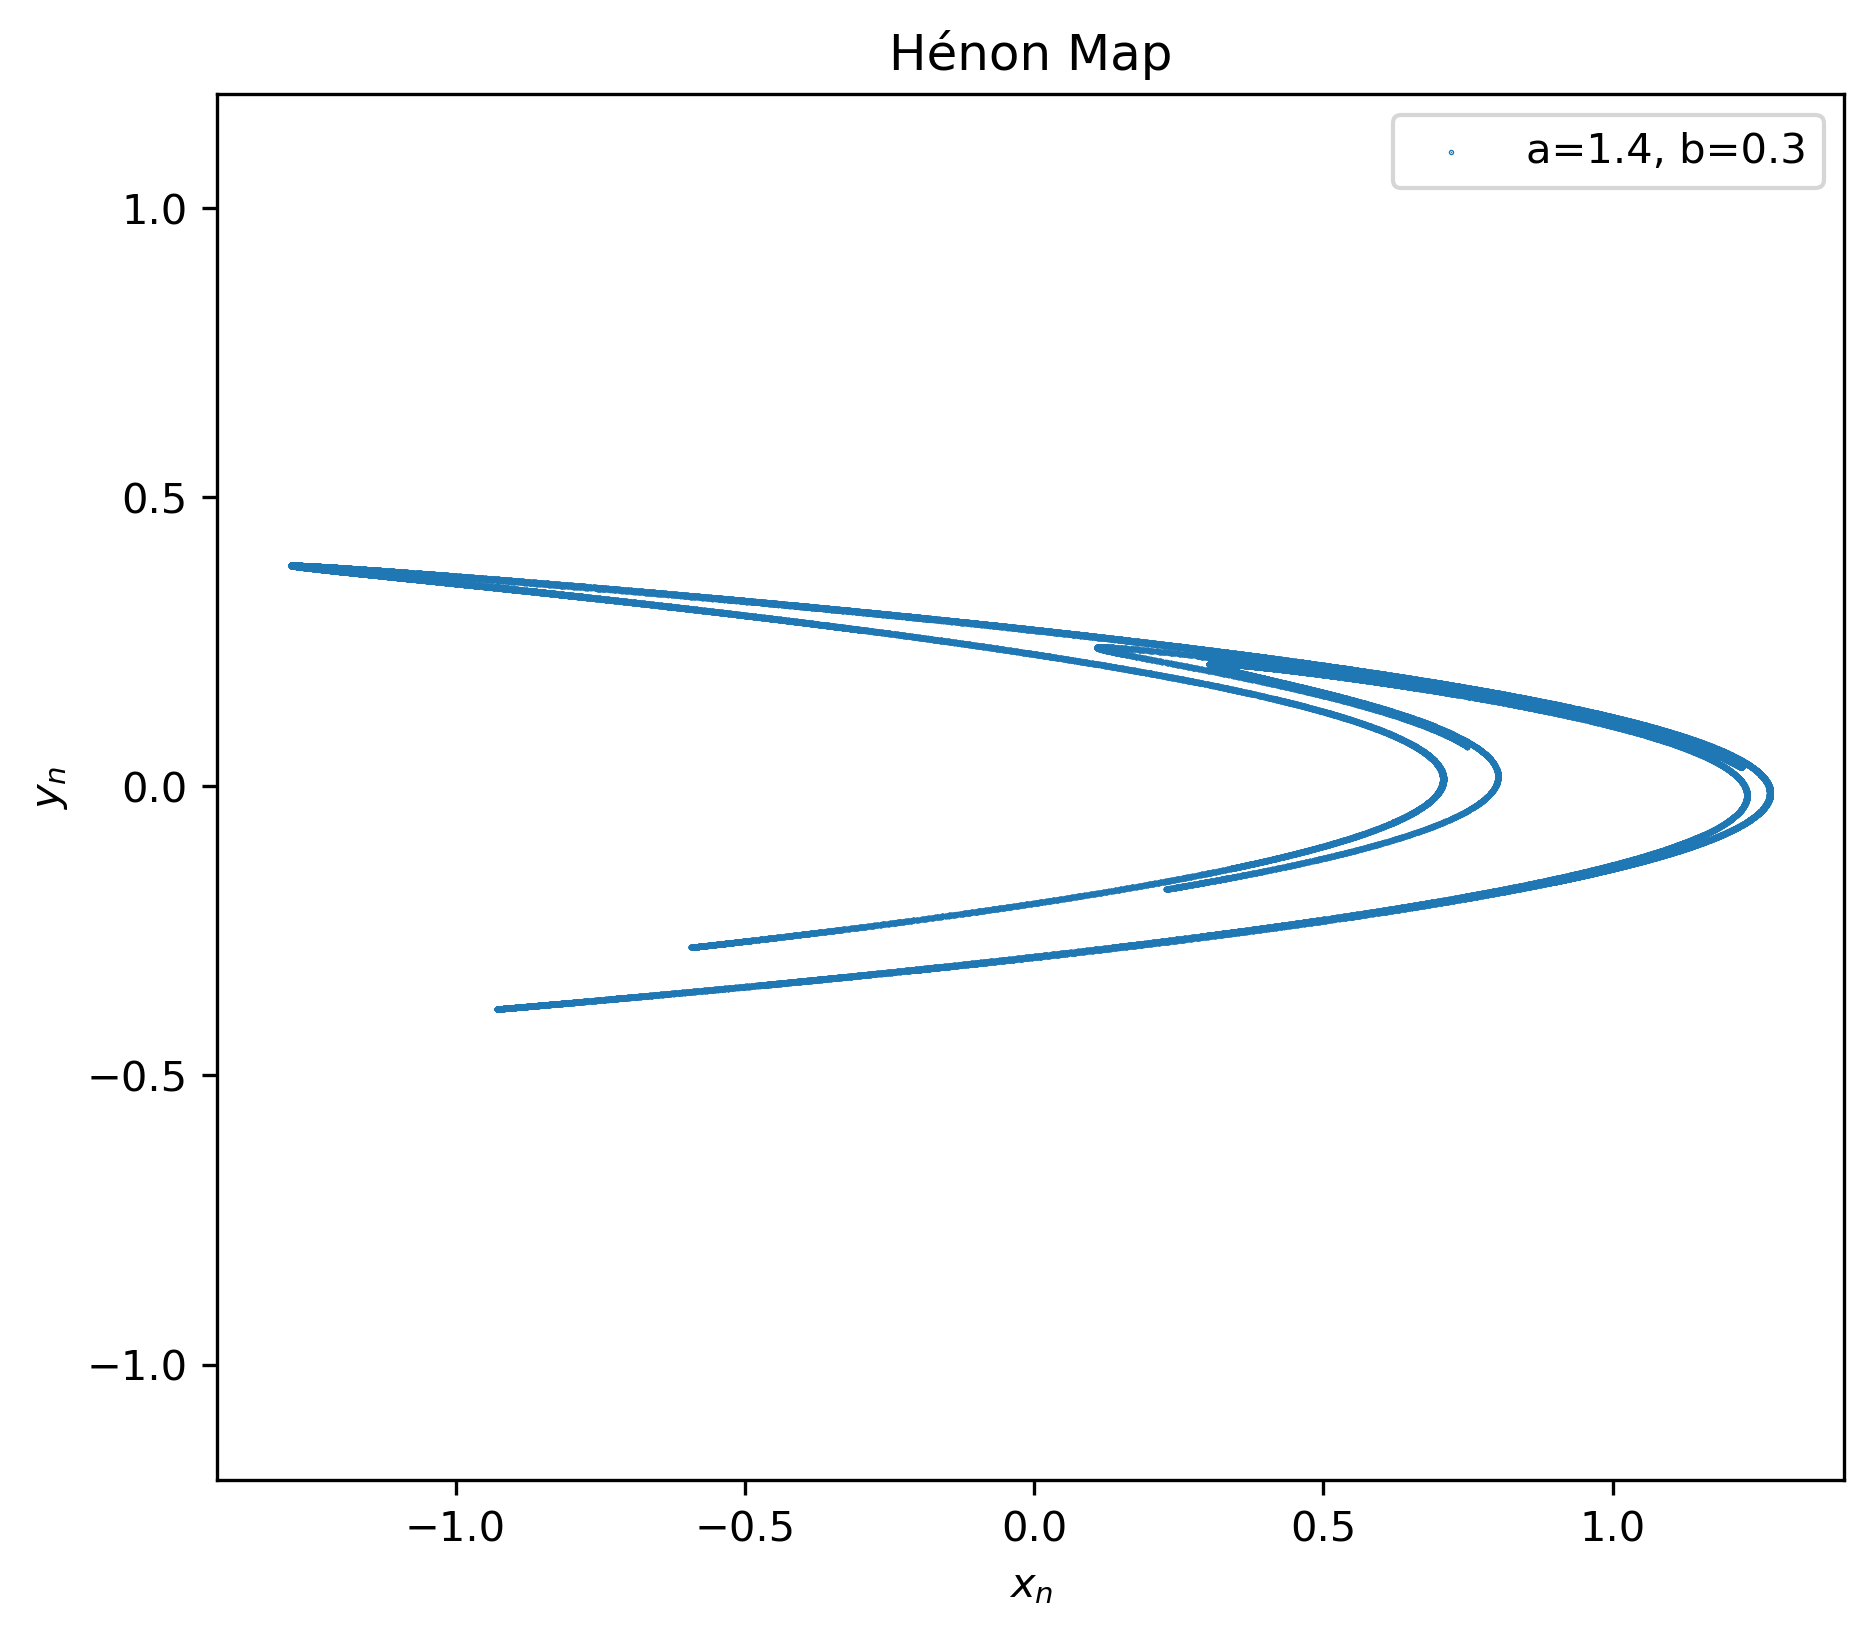
\includegraphics[width=0.7\textwidth]{graph_HenonMap.png}
\caption{Henon Map 에서 a=1.4,  b=0.3일때의 그래프를 나타낸다.}
\label{fig:graph}
\end{figure}

\vspace{1em}

1.4 Bifurcation diagram
\begin{figure}[H]
\centering
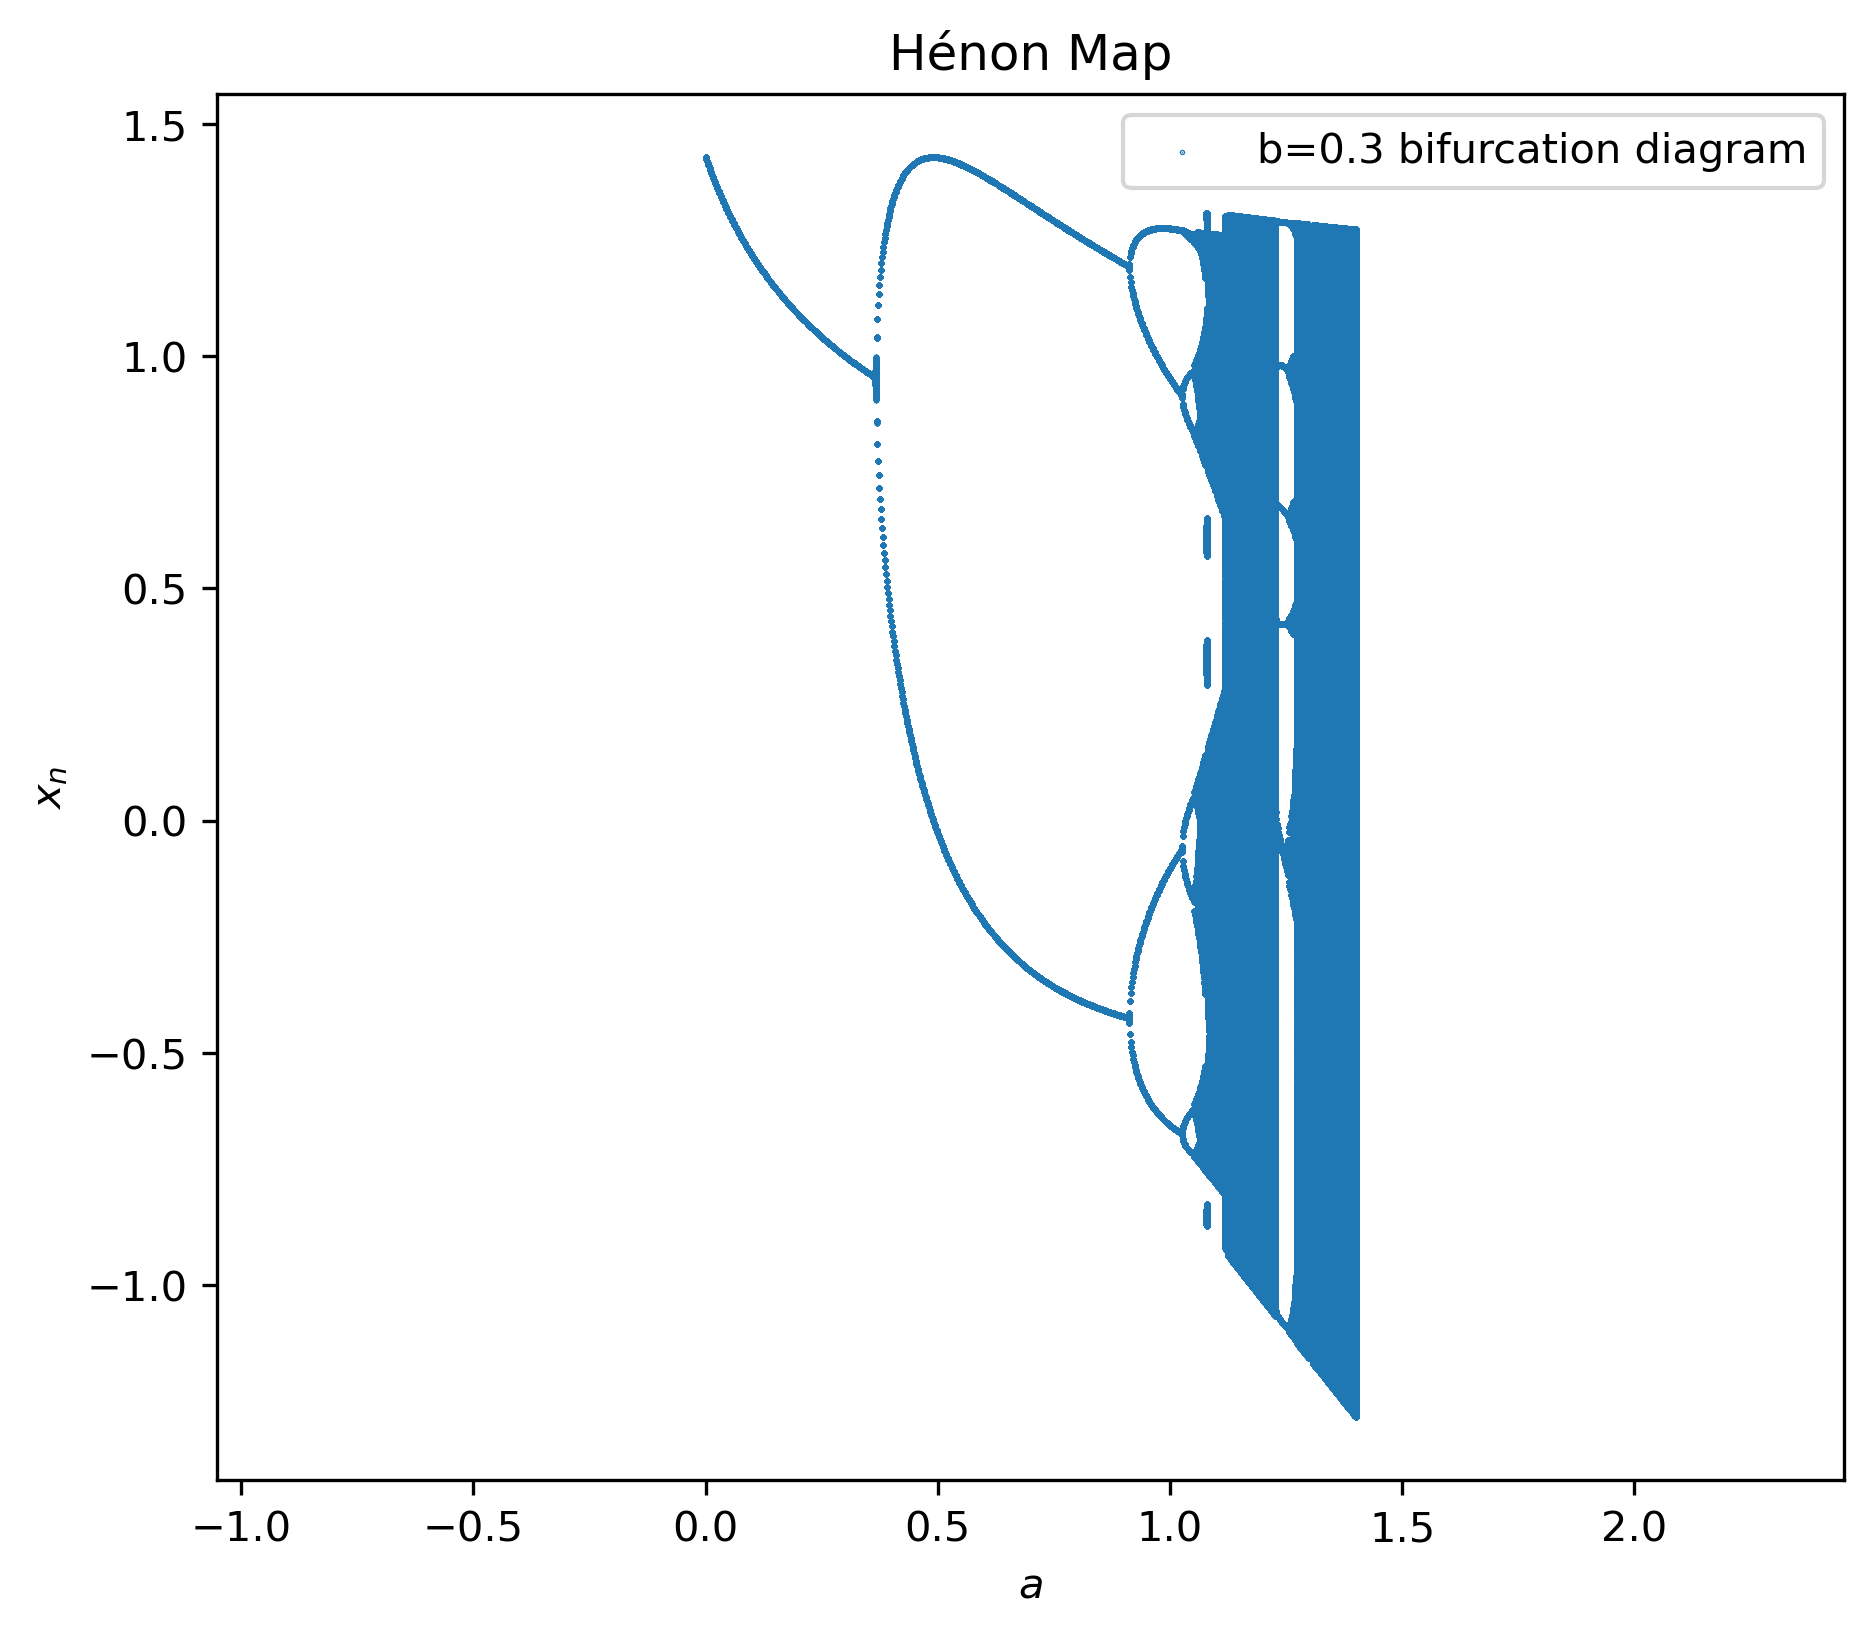
\includegraphics[width=0.7\textwidth]{graph_Bif.png}
\caption{b=0.3일때 a값에 따른 $x_n$의 갈래치기를 나타낸 그래프이다.}
\label{fig:graph_2}
\end{figure}

1.5 Chaos and Fractals

교재에서는 헤논맵에서 발생하는 카오스와 헤넌 어프렉터의 프렉탈 구조를 하나의 직사각형이 구부러지는 형태로 분석을 하였다.
\begin{figure}[H]
\centering

\begin{subfigure}{0.32\textwidth}
    \centering
    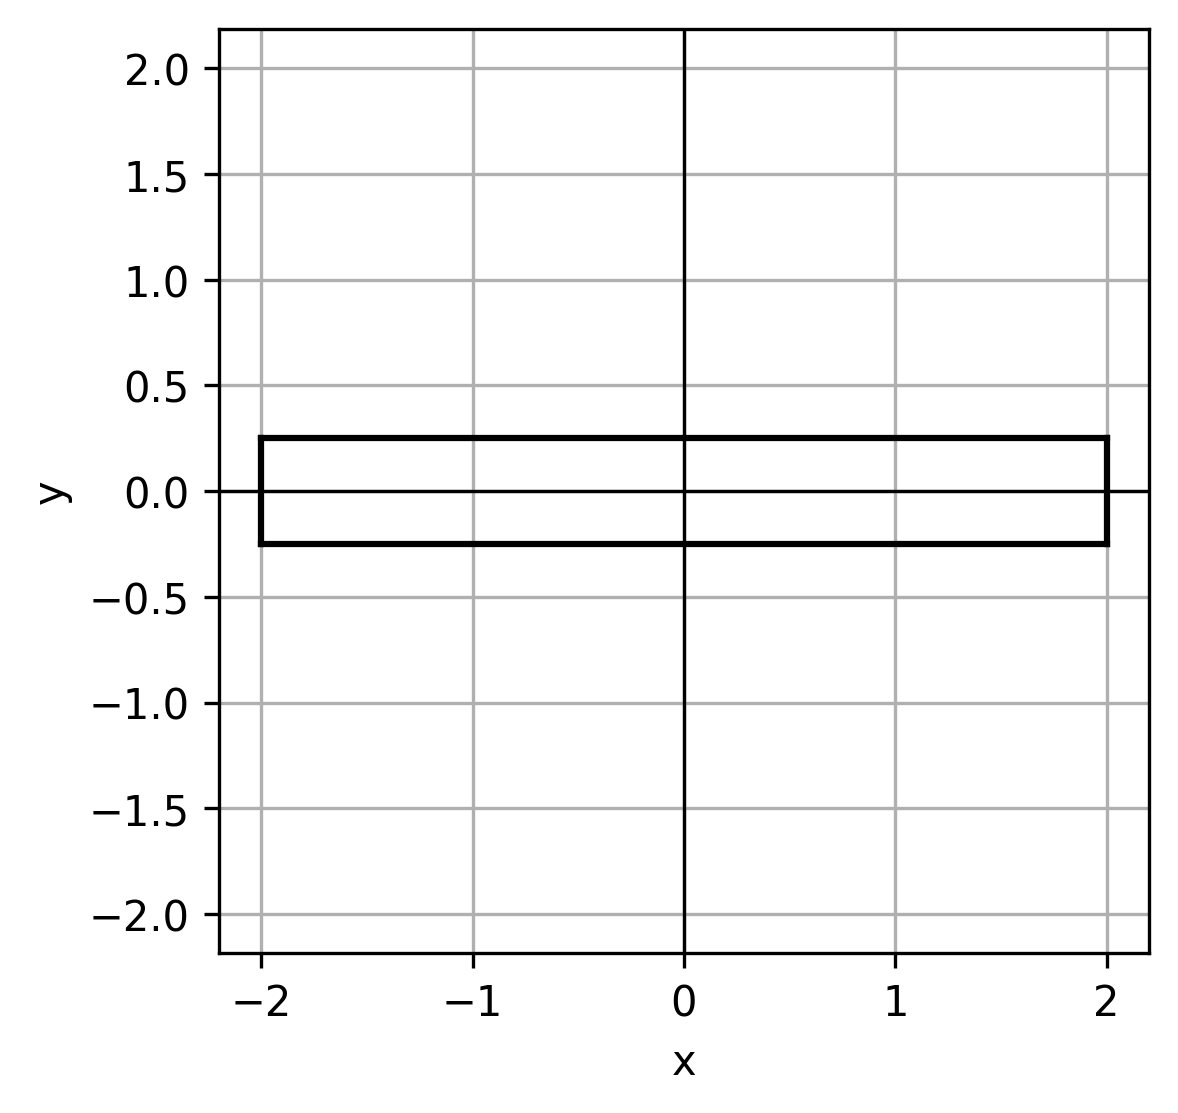
\includegraphics[width=\textwidth]{square.png}
    \caption{초기 사각형}
    \label{fig:square}
\end{subfigure}
\hfill
\begin{subfigure}{0.32\textwidth}
    \centering
    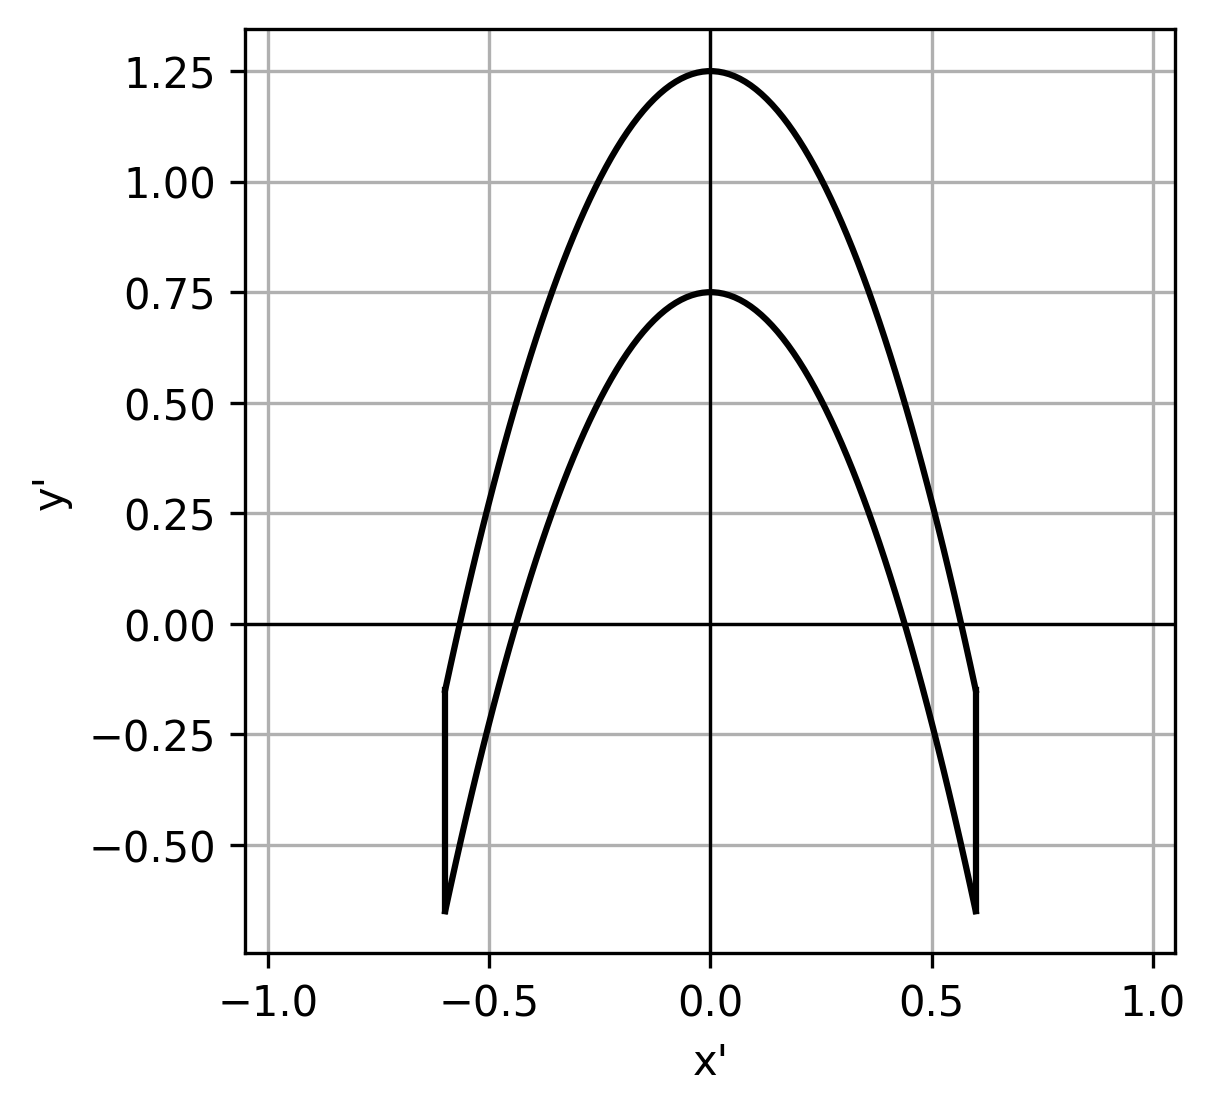
\includegraphics[width=\textwidth]{square_Fold.png}
    \caption{접힘 변환}
    \label{fig:square_fold}
\end{subfigure}
\hfill
\begin{subfigure}{0.32\textwidth}
    \centering
    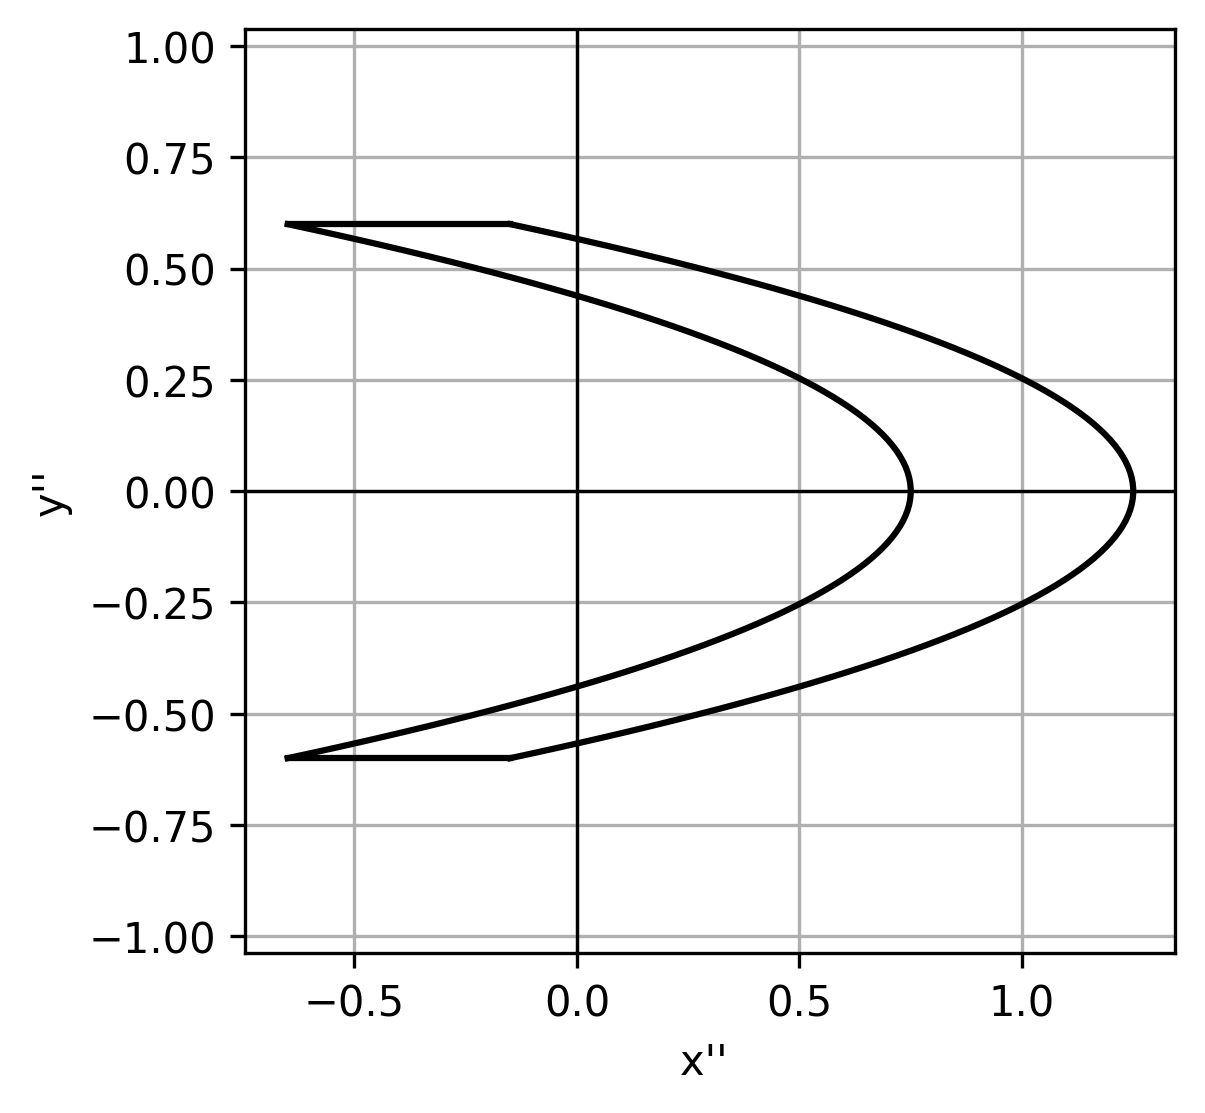
\includegraphics[width=\textwidth]{square_axis.png}
    \caption{축 변환 후 형태}
    \label{fig:square_axis}
\end{subfigure}

\caption{해논맵에서 사각형 영역이 접히고 수축되는 과정을 나타낸 그림이다.}
\label{fig:henon_square_transform}
\end{figure}

위 figure 3처럼 사각형을 휘고 돌리는 과정을 반복하면서 프렉탈 구조처럼 나타난다.
이 과정을 반복하면 그림 \ref{fig:graph}과 같은 형태로 그려지게 된다.


\end{document}